\documentclass[11pt,a4paper]{article}

\usepackage[utf8]{inputenc}
\usepackage[T1]{fontenc}
\usepackage[brazil]{babel}
\usepackage{amsmath,amssymb}
\usepackage{graphicx}
\usepackage{booktabs}
\usepackage{hyperref}
\usepackage[margin=2.5cm]{geometry}

\graphicspath{{../figures/}}

\title{Filtros Digitais para Processamento de Sinais Biom\'edicos:\\
um estudo comparativo de denoising de ECG}
\author{Equipe ES413 --- CIn/UFPE\\\small (Manoel \& equipe)}
\date{\today}

\begin{document}
\maketitle

\begin{abstract}
Este trabalho projeta, implementa e compara filtros digitais para a remo\c{c}\~ao de
tr\^es interfer\^encias t\'ipicas do eletrocardiograma (ECG): interfer\^encia da rede
el\'etrica ($60\,$Hz), varia\c{c}\~ao da linha de base ($0{,}05$--$0{,}5\,$Hz) e ru\'ido
muscular (EMG, $>40\,$Hz). Avaliam-se filtros convencionais (notch IIR, passa-alta
Butterworth e passa-baixa FIR de fase linear) e abordagens avan\c{c}adas/inteligentes
(filtro adaptativo LMS/NLMS, transformada wavelet discreta e \emph{autoencoder}
convolucional de denoising), sob um mesmo protocolo de contamina\c{c}\~ao controlada com as
bases p\'ublicas MIT-BIH \texttt{mitdb} e \texttt{nstdb} do PhysioNet.
\end{abstract}

\section{Introdu\c{c}\~ao}
O eletrocardiograma (ECG) registra a atividade el\'etrica do cora\c{c}\~ao e \'e o sinal
biom\'edico mais estudado em processamento digital de sinais, com componentes
morfol\'ogicos bem definidos --- ondas P, complexo QRS e onda T --- na faixa de
$0{,}05$--$150\,$Hz~\cite{rangayyan2024}. Sinais adquiridos em ambiente cl\'inico ou
ambulatorial est\~ao sujeitos a tr\^es classes principais de ru\'ido que comprometem a
an\'alise autom\'atica: a interfer\^encia da rede el\'etrica em $60\,$Hz, a deriva de baixa
frequ\^encia da linha de base e o artefato mioel\'etrico de alta frequ\^encia. A remo\c{c}\~ao
desses ru\'idos \'e pr\'e-requisito para qualquer an\'alise
automatizada~\cite{challis1982part1}.

Este projeto tem por objetivo (i) projetar e validar filtros convencionais que tratem
essas tr\^es classes de problema, explorando ferramentas do curso (transformada-z, DTFT,
equa\c{c}\~oes de diferen\c{c}as); (ii) projetar ao menos um filtro com t\'ecnicas
avan\c{c}adas/inteligentes; e (iii) realizar um estudo comparativo objetivo entre as
abordagens.

\section{Fundamenta\c{c}\~ao Te\'orica}

\subsection{Sinais discretos, DTFT e transformada-z}
Um sinal discreto $x[n]$ obtido por amostragem uniforme tem espectro dado pela
transformada de Fourier de tempo discreto (DTFT),
$X(e^{j\omega})=\sum_{n=-\infty}^{\infty}x[n]e^{-j\omega n}$, e \'e analisado no plano
complexo pela transformada-z, $X(z)=\sum_{n=-\infty}^{\infty}x[n]z^{-n}$, com
$z=e^{j\omega}$ sobre a circunfer\^encia unit\'aria. Os polos e zeros de $X(z)$ determinam
estabilidade e forma da resposta em frequ\^encia.

\subsection{Filtros IIR e FIR}
Um filtro IIR (recursivo) tem equa\c{c}\~ao de diferen\c{c}as e fun\c{c}\~ao de
transfer\^encia
\begin{equation}
y[n]=\sum_{k=0}^{M} b_k\,x[n-k]-\sum_{k=1}^{N} a_k\,y[n-k],
\qquad
H(z)=\frac{\sum_{k=0}^{M} b_k z^{-k}}{1+\sum_{k=1}^{N} a_k z^{-k}}.
\end{equation}
Um filtro FIR (n\~ao recursivo) depende apenas das entradas:
\begin{equation}
y[n]=\sum_{k=0}^{M-1} h[k]\,x[n-k],
\qquad
H(z)=\sum_{k=0}^{M-1} h[k] z^{-k}.
\end{equation}
A resposta em frequ\^encia \'e $H(e^{j\omega})=H(z)\big|_{z=e^{j\omega}}$. O FIR de
coeficientes sim\'etricos possui \emph{fase linear}, com atraso de grupo constante
$(M-1)/2$ amostras --- propriedade essencial para n\~ao distorcer as rela\c{c}\~oes
temporais entre as ondas P, QRS e T.

\subsection{Filtros convencionais para ECG}
\paragraph{Notch IIR ($60\,$Hz).} Filtro de rejei\c{c}\~ao de banda estreita
($\approx 2\,$Hz) centrado em $60\,$Hz, com fator de qualidade $Q=f_0/\mathrm{BW}=30$,
removendo a rede sem degradar o QRS. A Figura~\ref{fig:notch} mostra polos/zeros e
$|H(e^{j\omega})|$.
\paragraph{Passa-alta IIR Butterworth ($f_c=0{,}5\,$Hz).} Corrige a varia\c{c}\~ao da
linha de base preservando o segmento PR e o QRS; a resposta de magnitude maximamente plana
do Butterworth evita ondula\c{c}\~ao na banda de passagem~\cite{challis1983part3}.
\paragraph{Passa-baixa FIR Hamming ($f_c=40\,$Hz, 61 taps).} Atenua o ru\'ido muscular de
alta frequ\^encia; a janela de Hamming oferece atenua\c{c}\~ao de l\'obulo lateral de
$\approx -41\,$dB~\cite{challis1982part1}.

\begin{figure}[t]
  \centering
  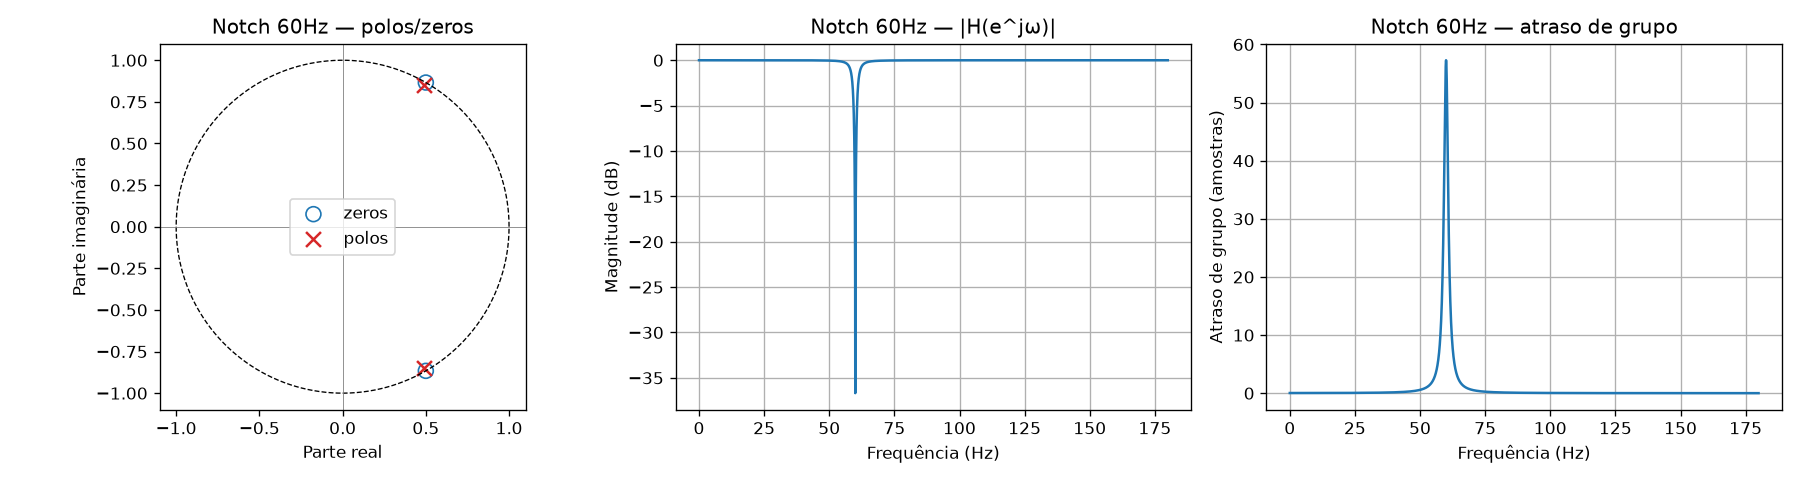
\includegraphics[width=\linewidth]{formalizacao_notch_60hz.png}
  \caption{Notch $60\,$Hz: diagrama de polos/zeros, $|H(e^{j\omega})|$ e atraso de grupo.}
  \label{fig:notch}
\end{figure}

\subsection{Filtro adaptativo LMS/NLMS}
O cancelamento adaptativo estima e subtrai a interfer\^encia a partir de uma
refer\^encia, ajustando os coeficientes em tempo real:
$\mathbf{w}[n+1]=\mathbf{w}[n]+\mu\,e[n]\,\mathbf{x}[n]$. Diferentemente do notch fixo,
acompanha flutua\c{c}\~oes de frequ\^encia/amplitude da rede, sendo adequado a sistemas
n\~ao estacion\'arios~\cite{widrow1975,thakor1991}.

\subsection{Transformada wavelet discreta (DWT)}
A DWT decomp\~oe o ECG em sub-bandas de aproxima\c{c}\~ao e detalhe (an\'alise
multirresolu\c{c}\~ao); o ru\'ido \'e atenuado por limiariza\c{c}\~ao
(\emph{soft-thresholding}) dos coeficientes de detalhe~\cite{donoho1995}, com wavelets-m\~ae
da fam\'ilia Daubechies (db4/db6) por sua semelhan\c{c}a morfol\'ogica com o
QRS~\cite{singh2006}.

\subsection{Autoencoder convolucional de denoising (DAE)}
Como t\'ecnica inteligente, um \emph{autoencoder} totalmente convolucional \'e treinado
para reconstruir o ECG limpo a partir de janelas contaminadas, tratando as tr\^es classes
de ru\'ido em um \'unico modelo n\~ao linear~\cite{chiang2019,romero2021}, alinhado \`a
tend\^encia apontada por~\cite{ferdous2023,tripathi2024}.

\section{Metodologia experimental}
Registros do \texttt{mitdb} ($f_s=360\,$Hz) s\~ao tratados como sinal de refer\^encia
(``limpo''); sobre eles somam-se, em n\'iveis de SNR controlados (0, 6, 12 e $18\,$dB), os
ru\'idos reais do \texttt{nstdb} (\texttt{bw}, \texttt{ma}, \texttt{em}) e a senoide de
$60\,$Hz~\cite{moody1984nstdb,goldberger2000}. Como o sinal limpo \'e conhecido,
calculam-se m\'etricas objetivas: melhoria de SNR (dB), RMSE, PRD e coeficiente de
correla\c{c}\~ao. Dois cuidados de protocolo: avaliar o FIR em fase-zero (ou compensar o
atraso de grupo) e, para a deriva de linha de base, usar uma refer\^encia tamb\'em
passa-alta.

% --- Se\c{c}\~oes a completar pela equipe (Etapas C/D): Resultados e Conclus\~ao ---
\section{Resultados}
\label{sec:resultados}
% Inserir a tabela comparativa (figures/comparacao_convencionais.csv) e as figuras
% antes/depois geradas por scripts/gerar_figuras.py.

\section{Conclus\~ao}
% A completar.

\bibliographystyle{ieeetr}
\bibliography{referencias}

\end{document}
